\begin{frame}{Was ist ein Embedded System?}
	Der Ausdruck embedded system bezeichnet einen Computer, der in einem technischen Kontext eingebettet ist. \cite{wikiEmbedded}
	\begin{flushright}
		Nach Wikipedia
	\end{flushright}
	
	Was macht ein Embedded System speziell \cite{embeddedSpecials}
	\begin{itemize}
		\item Echtzeit
		\item Grösse
		\item Kosten
		\item Zeit
		\item Zuferlässigkeit
		\item Sicherheit
		\item Energy
		\item Langlebigkeit
	\end{itemize}
\end{frame}

\begin{frame}{grosses Embedded System: ATLAS/LHC/CERN}
	\begin{center}
		\begin{tabular}{cc}
			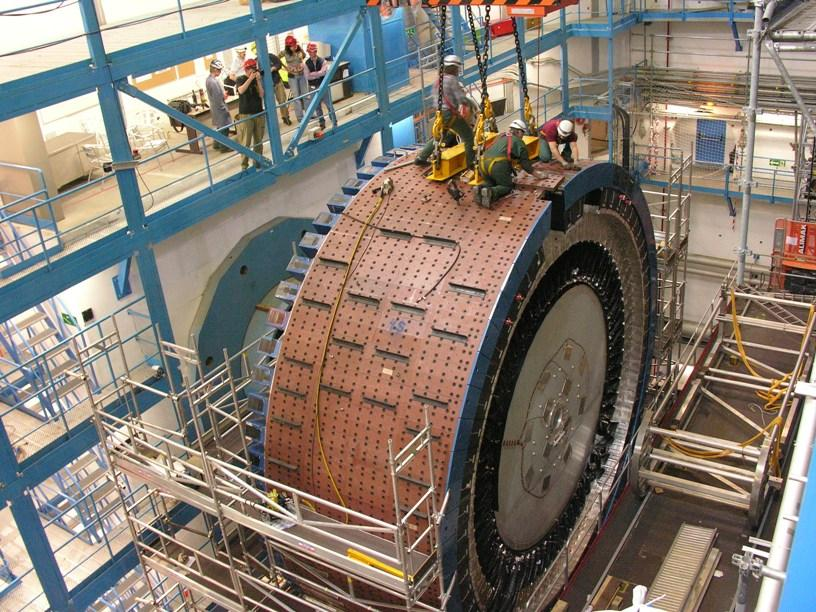
\includegraphics[height=4cm]{res/ATLAS_Tile_Calorimeter} &  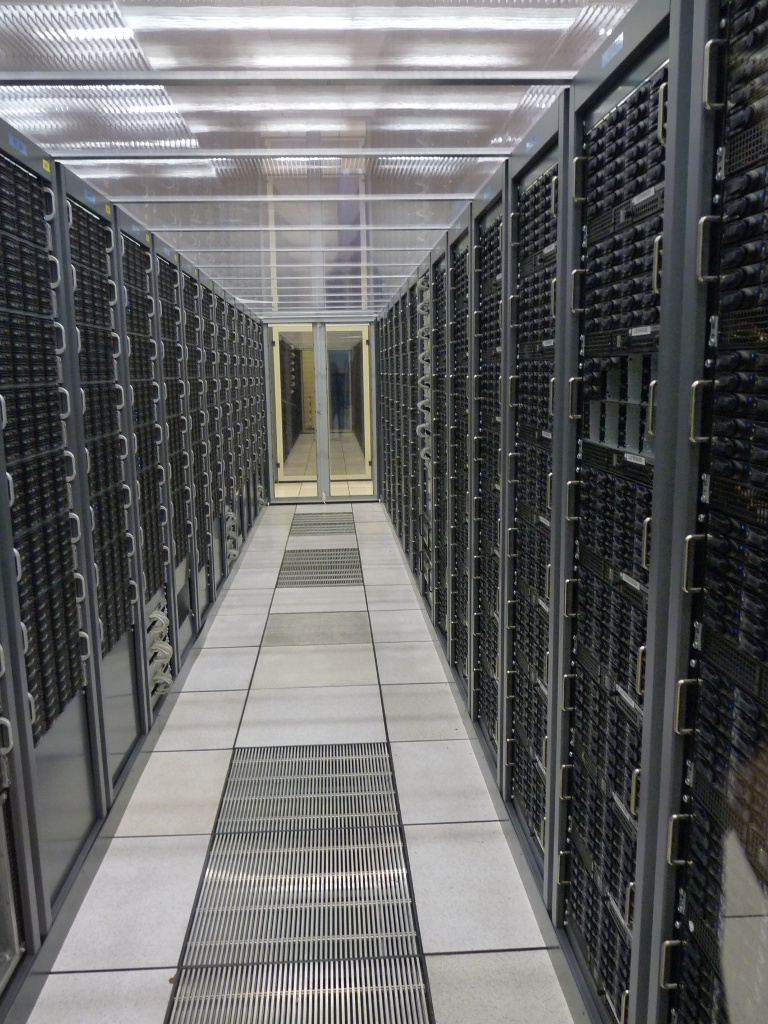
\includegraphics[height=4cm]{res/CERN_server.jpg} \\ 
			cc-by-sa-2.0 Argonne National Laboratory & cc-by-sa Urs Fässler \\
		\end{tabular} 
	\end{center}
	\begin{itemize}
		\item Sensor produziert 1 petabyte Daten pro Sekunde
		\item Systems verarbeitet dies auf etwas mehr als 100 MB pro Sekunde \cite{wikiAtlas}
		\item Verarbeitung auf eigenen 20'000 Server und Grid \cite{wikiCernServer}
	\end{itemize}
\end{frame}

\begin{frame}{prototypisches GNU/Linux Embedded System}
	Raspberry PI
	BeagleBone
\end{frame}

\begin{frame}{Echtzeit}
	\begin{itemize}
		\item Bearbeitung ist nach einer bestimmten Zeit nach dem auftreten eines Ereignisses abgeschlossen.
		\item Die Bearbeitung eines Interrupts dauert nie laenger als $t$.
		\item bei weicher Echtzeit ist dieses Verhalten wuenschenswert (Video wiedergabe)
		\item jeder Treiber kann Interrupts sperren
		\item Swapping
		\item Prozessoren mit Caches haben undefinierbares Verhalten, abschalten nicht Sinn der Sache
		\item Loesung ist separater uC, im selben oder eigenen DIE
	\end{itemize}
\end{frame}


